%  !TeX  root  =  user_guide.tex
%%\author{1.0.0 traduit par Jérémy Garniaux, 1.3.0 par Marie Silvestre}


%\section{\qg Plugins}\label{sec:plugins}\index{plugins}
\chapter{Les extensions de \qg}\label{sec:extensions}\index{extensions}

% when the revision of a section has been finalized, 
% comment out the following line:
%\updatedisclaimer

%\qg has been designed with a plugin architecture.
%This allows new features/functions to be easily added to the application.
%Many of the features in \qg are actually implemented as \textbf{core} or \textbf{external} plugins.\index{plugins!types} 

\qg repose sur un système d'extensions. Ce dernier permet d'ajouter facilement de nouvelles fonctions au logiciel.  De nombreuses nouvelles fonctions de \qg sont implémentées comme des extensions \textbf{principales} ou \textbf{complémentaires}. \index{plugins!types} 

\begin{itemize}[label=--]
%\item \textbf{Core Plugins} are maintained by the \qg Development Team and are automatically part of every \qg distribution.
%They are written in one of two languages: C++ or Python.
%More information about core plugins are provided in Section \ref{sec:core_plugins}.
%\item \textbf{External Plugins} are currently all written in Python.
%They are stored in external repositories and maintained by the individual authors.
%They can be added to \qg using the \filename{Plugin Installer}.
%More information about external plugins are provided in Section \ref{sec:external_plugins}.
\item Les \textbf{extensions principales} sont maintenues par l'équipe de développement de \qg et sont intégrées automatiquement à chaque nouvelle distribution de \qg. Elles sont écrites en C++ ou en Python. On trouvera plus d'informations sur les extensions principales dans la Section \ref{sec:core_plugins}.
\item Les \textbf{extensions complémentaires} sont actuellement toutes écrites en Python. Elles sont stockées dans des dépôts externes et maintenues par leurs auteurs. Elles peuvent être ajoutées à \qg en utilisant le \filename{Gestionnaire d'extensions}. On trouvera plus d'informations sur les extensions complémentaires dans la Section \ref{sec:external_plugins}.
\end{itemize}

%\section{Managing Plugins}\label{sec:managing_plugins}
%\index{plugins!managing} 
\section{Gérer les extensions}\label{sec:managing_plugins}
\index{plugins!managing} 

%Managing plugins in general means loading or unloading them using
%the \filename{Plugin Manager}. External plugins can be installed and
%directly activated or uninstalled using the \filename{Python Plugin
%Installer}. To deactivate and reactivate external plugins, the
%\filename{Plugin Manager} is used again.
De manière générale, gérer les extensions consiste à les afficher ou pas à l'aide du \filename{Gestionnaire d'extension}.
Les extensions complémentaires doivent d'abord être installées à l'aide de \filename{Installateur d'extensions python} pour pouvoir être activées ou désactivées dans le \filename{Gestionnaire d'extension}.

%\subsection{Loading a \qg Core Plugin}\label{sec:load_core_plugin} 
\subsection{Installer une extension principale}\label{sec:load_core_plugin} 

%Loading a \qg Core Plugin is done from the main menu \mainmenuopt{Plugins} > \dropmenuopttwo{mActionShowPluginManager}{Manage Plugins...}.\index{plugins!manager}
On active une extension principale à l'aide du menu\\ \mainmenuopt{Extensions} > \dropmenuopttwo{mActionShowPluginManager}{Gestionnaire d'extension\dots}.\index{plugins!manager}

\begin{figure}[ht]
   \begin{center}
%   \caption{Plugin Manager \nixcaption}\label{fig:pluginmanager}\smallskip 
   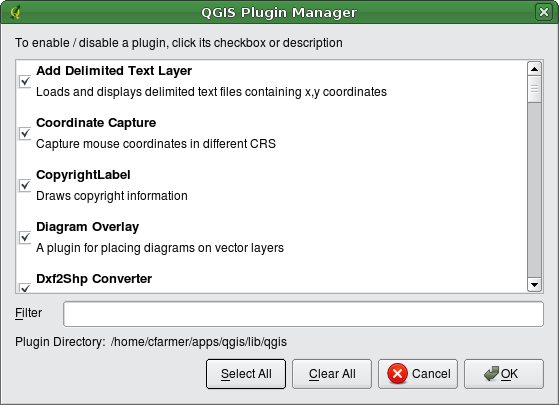
\includegraphics[clip=true, width=12cm]{pluginmanager}
   \caption{Gestionnaire d'extension \nixcaption}\label{fig:pluginmanager}
\end{center}
\end{figure}

%The \filename{Plugin Manager} lists all the available plugins and their status (loaded or unloaded), 
%including all core plugins and all external plugins that have been added using the \filename{Plugin Installer} 
%(see Section \ref{sec:external_plugins}). Those plugins that are already loaded have a check mark 
%to the left of their name. Figure \ref{fig:pluginmanager} shows the Plugin Manager dialog.
Le gestionnaire d'extension liste toutes les extensions disponibles et leur statut (installé ou pas), dont toutes les extensions principales et toutes celles complémentaires que vous avez ajoutées à l'aide du \filename{Gestionnaire d'Extension} (voir Section \ref{sec:external_plugins}). Les extensions installées sont cochées à gauche de leur nom. La figure \ref{fig:pluginmanager} montre la boîte de dialogue du Gestionnaire d'extension.

%To enable a particular plugin, click on the checkbox to the left of the plugin name, and click \button{OK}. 
%When you exit the application, a list of loaded plugins is retained, and the next time 
%you run \qg these plugins are automatically loaded.
Pour installer une extension, cocher la case à gauche du nom puis cliquez sur \button{OK}. Les extensions installées sont mémorisées lorsque vous quittez l'application et seront restaurées à la prochaine ouverture de \qg.

%\begin{Tip}\caption{\textsc{Crashing Plugins}}\index{crashes}
%\qgistip{If you find that \qg crashes on startup, a plugin may be at fault.
%You can stop all plugins from loading by editing your stored settings file (see \ref{subsec:gui_options} for location).
%Locate the plugins settings and change all the plugin values to false to prevent them from loading.
%\nix {For example, to prevent the Delimited text plugin from loading, the entry in \$HOME/.config/QuantumGIS/qgis.conf on Linux should look like this:\usertext{Add Delimited Text Layer=false}.}
%\normalfont 
%Do this for each plugin in the [Plugins] section.
%You can then start \qg and add the plugins one at a time from the \filename{Plugin Manager} to 
%determine which plugin is causing the problem.}
%\end{Tip} 
\begin{Tip}\caption{\textsc{Extensions et plantages}}\index{crashes}
Si votre installation de \qg plante au démarrage, une extension est peut-être en cause. Vous pouvez éviter le chargement des extensions en éditant votre fichier de configuration (voir \ref{subsec:gui_options} pour localiser ce fichier). Localisez la configuration de l'extension et changez toutes les valeurs à \og false\fg pour empêcher leur chargement. \nix {Par exemple, pour éviter le chargement de l'extension \og Ajouter une couche texte délimité\fg, sa référence dans \$HOME/.config/QuantumGIS/qgis.conf doit ressembler à \usertext{Add Delimited Text Layer=false}.} Faites de même pour chaque extension dans la section [Extension]. Vous pouvez ensuite démarrer \qg et ajouter les extensions une à la fois depuis le \filename{Gestionnaire d'extension} pour déterminer celle qui est la source du problème.
\end{Tip}


%\subsection{Loading an external \qg Plugin}\label{sec:load_external_plugin} 
\subsection{Installer une extension externe de \qg}\label{sec:load_external_plugin} 

%There are two steps required to integrate external plugins into \qg: 
Une seule étape est nécessaire pour installer une extension externe dans \qg :

\begin{enumerate}
%\item Download an external plugin from a repository using the
%\filename{Python Plugin Installer} (Section \ref{sec:python_plugin_installer}).
%The new external plugin will be added to the list of available plugins in
%the \filename{Plugin Manager} and is automatically loaded.
\item Télechargez une extension externe depuis un dépôt à l'aide de l'\filename{Installeur d'extension python} (Section \ref{sec:python_plugin_installer}). La nouvelle extension complémentaire sera ajoutée à la liste des extensions disponibles dans le \filename{Gestionnaire d'extension} et automatiquement chargée dans \qg.
\end{enumerate}

%\subsection{Using the \qg Python Plugin Installer}\index{plugins!installing}\label{sec:python_plugin_installer}
\subsection{Utiliser l'installeur d'extension python de \qg}\index{plugins!installing}\label{sec:python_plugin_installer}
\index{plugins!Python Plugin Installer}\index{plugins!upgrading}

\begin{figure}[ht]
   \begin{center}
%   \caption{Installing external python plugins \nixcaption}
   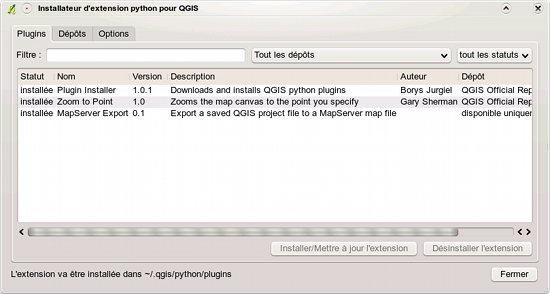
\includegraphics[clip=true, width=12cm]{plugininstaller}
   \caption{Installer des extensions python complémentaires\nixcaption}
\label{fig:plugininstaller}
\end{center}
\end{figure}

%In order to download and install an external Python plugin, click the menu \mainmenuopt{Plugins} > \dropmenuopttwo{plugin_installer}{Fetch Python Plugins...}.
Pour télécharger et installer une extension python complémentaire, cliquez sur le menu\\ \mainmenuopt{Extensions} > \dropmenuopttwo{plugin_installer}{Récupération des extensions python.\dots}.
%The \filename{Plugin Installer} window will appear (figure \ref{fig:plugininstaller}) with the tab \tab{Plugins}, containing a list of all locally installed Python plugins, as well as plugins available in remote repositories. Each plugin can be either:
La fenêtre de l'\filename{Installeur\\ d'extension python} apparaîtra (figure \ref{fig:plugininstaller}) avec l'onglet \tab{Extensions}, qui présente la liste de toutes les extensions python installées localement ou disponibles dans des dépôts distants. Chaque extension peut-être soit :

\begin{description}
%\item \textbf{not installed} - this means the plugin is available in the repository, but is not installed yet. In order to install it, select the plugin from the list and click the \button{Install plugin} button.
%\item \textbf{new} - this means that the plugin is newly available in the repository.
%\item \textbf{installed} - this indicates that the plugin is already installed. If it is also available in any repository the \button{Reinstall plugin} button will be enabled. If the available version is older than the installed version, the \button{Downgrade plugin} button will appear instead.
%\item \textbf{upgradeable} - this means that the plugin is installed, but there is an updated version available. In this case, the \button{Upgrade plugin} button will be enabled.
%\item \textbf{invalid} - this means that the plugin is installed, but is unavailable or broken. The reason will be explained in the plugin description field.
\item[non installée :]signifie que l'extension est disponible dans le dépôt, mais n'est pas encore installée. Pour l'installer, sélectionnez-la dans la liste et cliquez sur le bouton\\ \button{Installer l'extension}
\item[nouveau :] signifie que l'extension est nouvelle dans le dépôt
\item[installée :] l'extension est déjà installée. Si elle est également disponible dans un dépôt, le bouton \button{Ré-installer l'extension} est actif. En revanche, si la version disponible est plus ancienne que la version installée, le bouton \button{Rétrograder la version} apparaît à la place
\item[mise à jour :] l'extension est installée, mais une version plus récente est disponible. Le bouton \button{Mise à jour de l'extension} est actif.
\item[invalide :] l'extension est installée, mais ne fonctionne pas. Les détails sont donnés dans la description de l'extension
\end{description}

%\minisec{Plugins tab}
\minisec{Onglet Extensions}

%To install a plugin, select it from the list and click the \button{Install plugin} button. The plugin is installed in its own directory. 
Pour installer une extension, sélectionnez-la dans la liste et cliquez sur le bouton\\ \button{Installer l'extension}. L'extension est installée dans un répertoire qui lui est dédié, cet emplacement diffère selon les systèmes d'exploitation :

\begin{itemize}[label=--]
%\item \nix{Linux and other unices}:\\
%./share/qgis/python/plugins \\
%/home/\$USERNAME/.qgis/python/plugins
%\item \osx{Mac OS X}:\\
%./Contents/MacOS/share/qgis/python/plugins \\
%/Users/\$USERNAME/.qgis/python/plugins
%\item \win{Windows}:\\
%C:\textbackslash Program Files\textbackslash \qg\textbackslash
%python\textbackslash plugins \\
%C:\textbackslash Documents and Settings\textbackslash\$USERNAME\textbackslash
%.qgis\textbackslash python\textbackslash plugins
\item \nix{Linux et autres unix} :\\
./share/qgis/python/plugins \\
/home/\$USERNAME/.qgis/python/plugins
\item \osx{Mac OS X} :\\
./Contents/MacOS/share/qgis/python/plugins \\
/Users/\$USERNAME/.qgis/python/plugins
\item \win{Windows} :\\
C:\textbackslash Program Files\textbackslash \qg\textbackslash
python\textbackslash plugins \\
C:\textbackslash Documents and Settings\textbackslash\$USERNAME\textbackslash
.qgis\textbackslash python\textbackslash plugins
\end{itemize}

%If the installation is successful, a confirmation message will appear.
Si l'installation est réussie, un message de confirmation apparaît.


%If the installation fails, the reason for the failure will be displayed
%in a warning dialog. Most often, errors are the result of connection problems
%and/or missing Python modules. In the former case you will likely need to
%wait before trying the install again, in the latter case, you should install
%the missing modules relevant to your operating system prior to using the
%plugin. \nix{For Linux, most required modules should be available via a
%package manager}. \win{For install instructions in Windows visit the module
%home page}. If you are using a proxy, you may need to configure it under
%\mainmenuopt{Edit} \arrow \dropmenuopttwo{mActionOptions}{Options} (Gnome, OSX)
%or \mainmenuopt{Settings} \arrow \dropmenuopttwo{mActionOptions}{Options} (KDE, Windows)
%on the \tab{Proxy} tab.

Si l'installation ne fonctionne pas, la raison est alors indiquée dans une fenêtre d'alerte. Les problèmes les plus fréquents sont dus à des erreurs de connexion et à des modules Python manquants. Dans le premier cas, il vous faudra probablement attendre quelques instants puis retenter l'installation (dans le cas où il s'agit d'un problème dû au serveur); dans le second cas, il sera nécessaire d'installer les modules manquants pour votre système d'exploitation avant d'utiliser les extensions. \nix{Pour Linux, la plupart des modules requis devraient être disponibles dans le gestionnaire de paquets de votre distribution}. \win{Pour les instructions d'installation pour Windows, visitez la page web du module}. Si vous utilisez un proxy, vous pourriez avoir besoin de le configurer dans le menu \mainmenuopt{Édition} > \dropmenuopttwo{mActionOptions}{Options} (Gnome, OSX) ou dans \mainmenuopt{Préférences} > \dropmenuopttwo{mActionOptions}{Options} (KDE, Windows) dans l'onglet \tab{Proxy}.

%The \button{Uninstall plugin} button is enabled only if the selected plugin is installed and is not a core plugin. Note that if you have installed an update to a core plugin, you can uninstall this update with the \button{Uninstall plugin} and revert to the version shipped with Quantum GIS. This default version however, cannot be uninstalled.
Le bouton \button{Désinstaller l'extension} est actif seulement si l'extension sélectionnée est installée et n'est pas une extension principale. Notez que si vous avez installé une mise à jour d'une extension principale, vous pouvez désinstaller cette mise à jour avec le bouton\\ \button{Désinstaller l'extension} et revenir à la version d'origine fournie à l'installation de Quantum GIS. Cette dernière ne peut pas être désinstallée.

%\minisec{Repositories tab}
\minisec{Onglet Dépôts}

%The second tab \tab{Repositories}, contains a list of plugin repositories available for the \filename{Plugin Installer}. By default, only the \qg Official Repository is enabled. You can add several user-contributed repositories, including the central \qg Contributed Repository and other external repositories by clicking the \button{Add 3rd party repositories} button. The added repositories contain a large number of useful plugins which are not maintained by the \qg Development Team. As such, we cannot take any responsibility for them. You can also manage the repository list manually, that is add, remove, and edit the entries. Temporarily disabling a particular repository is possible by clicking the \button{Edit...} button.
Le second onglet, \tab{Dépôts}, contient une liste de dépôts d'extensions disponibles pour l'\\\filename{Installateur d'extensions}. Par défaut, seul le Dépôt Officiel de \qg (\qg Official Repository) est utilisé. Vous pouvez ajouter des dépôts contenant des contributions d'utilisateurs, notamment le dépôt central de contributions de \qg (\qg Contributed Repository) et quelques autres dépôts externes cliquant sur le bouton \button{Ajouter un dépôt-tiers d'extension à la liste}. Ces dépôts contiennent une grande quantité d'extensions utiles, mais elles ne sont pas maintenues par l'équipe de développement de \qg et nous ne pouvons prendre aucune responsabilité les concernant. Vous pouvez également gérer la liste de dépôts manuellement, pour ajouter, retirer ou éditer des entrées. Désactiver temporairement un dépôt particulier est possible en cliquant sur le bouton \button{Éditer...}.


%\minisec{Options tab}
\minisec{Onglet Options}

%The \tab{Options} tab is where you can configure the settings of the \filename{Plugin Installer}. The \checkbox{Check for updates on startup} checkbox tells \qg to automatically look for plugin updates and news. By default, if this feature is enabled all repositories listed and enabled in the \tab{Repositories} tab are checked for updates each time the program is started. The frequency of update checking can be adjusted using the dropdown menu, and may be adjusted from once a day right up to once a month. If a new plugin or update is available for one of the installed plugins, a notification will appear in the Status Bar. If the checkbox is disabled, looking for updates and news is performed only when the \filename{Plugin Installer} is manually launched from the menu.
L'onglet \tab{Options} vous permet de configurer les paramètres de l'\filename{Installateur d'extensions}. La case \checkbox{Chercher des mises à jour au démarrage} configure \qg pour rechercher automatiquement les mises à jour et les actualités relatives aux extensions. Si la case est cochée, tous les dépôts listés et activés dans l'onglet \tab{Dépôts} sont vérifiés à chaque démarrage du programme. La fréquence de cette vérification peut être ajustée dans le menu déroulant allant d'une fois par jour à tous les mois. Si une nouvelle extension ou une mise à jour est disponible pour une des extensions installées, une notification cliquable apparaît dans la barre de statut. Si la case est décochée, la recherche de mises à jour et d'actualités s'effectue uniquement lorsque l'Installateur d'Extension est lancé manuellement depuis le menu.

%Although the plugin installer update can handle ports different from 80, some internet
%connections will cause problems when attempting to automatically check for updates.
%In these cases, a \textit{Looking for new plugins...} indicator will
%remain visible in the Status Bar during your entire QGIS session, and may cause a
%program crash when exiting. In this case please disable the checkbox.
Bien que l'installateur d'extensions puisse prendre en charge des ports autres que le 80, certaines connexions Internet peuvent poser des problèmes lors des vérifications automatiques. Dans ce cas, un indicateur \textit{Recherche de nouvelles extensions...} reste visible dans la barre de statut durant toute la session \qg et peut faire planter le programme à la fermeture. Dans ce cas, décochez la case.

%In addition, you may specify the type of plugins that are displayed by the \filename{Plugin Installer}. Under \textit{Allowed plugins}, you can specify whether you would like to:
De plus, vous pouvez spécifier le type d'extension qui sont affichées dans l'\filename{Installateur d'extensions}. Sous \textit{Extensions autorisées},vous pouvez spécifier si vous souhaitez :

\begin{itemize}[label=--]
%\item Only show plugins from the official repository
%\item Show all plugins except those marked as experimental,
%\item or Show all plugins, even those marked as experimental.
\item afficher seulement les extensions du dépôt officiel,
\item afficher toutes les extensions à l'exception de celles encore expérimentales,
\item afficher toutes les extensions, même celles encore expérimentales.
\end{itemize}

\begin{Tip}
% \caption{\textsc{Using experimental plugins}}
 \caption{\textsc{Utiliser des extensions expérimentales}}

%Experimental plugins are generally unsuitable for production use. These plugins are in the early stages of development, and should be considered 'incomplete' or 'proof of concept' tools. The \qg development team does not recommend installing these plugins unless you intend to use them for testing purposes.
Les extensions expérimentales sont généralement inadaptées à une utilisation en production. Ces extensions sont à des stades peu avancés de développement et doivent être considérées comme des outils 'incomplets' ou des 'démonstrations de faisabilité'. L'équipe de développement de \qg ne recommande pas de les installer sauf pour des besoins de test.
\end{Tip}


%\section{Data Providers}\index{data providers}
\section{Fournisseurs de données}\index{data providers}

%Data Providers are "special" plugins that provides access to a data store.
%By default, \qg supports PostGIS layers and disk-based data stores supported by the GDAL/OGR library (Appendix \ref{appdx_ogr}).
%A Data Provider plugin extends the ability of \qg to use other data sources.

%Data Provider plugins are registered automatically by \qg at startup.
%They are not managed by the Plugin Manager but used behind the scenes when a data type is added as a layer in \qg.
Les Fournisseurs de données sont des extensions "spéciales" donnant accès à un dépôt de données.
Par défaut, \qg supporte les couches PostGIS et les bases de données couvertes par la bibliothèque GDAL/OGR(Appendix \ref{appdx_ogr}).
L'utilisation d'extensions pour fournir des données permet d'élargir les sources de données utilisables par \qg.

Les extensions fournissant des données sont automatiquement enregistrées par \qg au démarrage.
Elles ne sont pas gérées par le Gestionnaire d'Extension, mais utilisées en arrière-plan lorsqu'un type de données est ajouté comme couche dans \qg.
